\documentclass[UTF8, twocolumn ]{ctexart}
\usepackage{graphicx}
\usepackage{amsmath}
\usepackage{amssymb}
\usepackage{paralist}
\usepackage[
  colorlinks,
  linkcolor = black
]{hyperref}

\usepackage{fancyhdr}                                
\usepackage{lastpage}                                           
\usepackage{layout}                                                                          

\linespread{1.56}
\columnsep = 15pt
\columnseprule=1pt
\begin{document}

\title{\huge{基于正态分布概率计算和支持向量机计算的WiFi定位技术}}
\author{北京优锐科技有限公司\ 丁贵金\ 朱韬\ 袁万尚}
%\author{北京优锐科技有限公司\ 朱韬}
\date{\today\\*\ \hrule}
\maketitle

%%%%%%%%%%%%%%%%%%%%%%%%%%%%%%%%%%%%%%%%%%%%%%%

\begin{abstract}
  基于正态分布概率和支持向量机原理的WiFi定位技术,完全采用软件科学计算方式来实现。该技术不需要依赖专用设备,部署简单使用便捷,对环境无强制依赖,可以在复杂WiFi环境下实现移动设备精确定位。该WiFi定位技术的核心原理是支持向量机,辅助计算的数学工具是正态分布的概率模型。整体技术框架为,采用正态分布概率模型筛选校准信息,同时确定移动设备大致方位,之后将筛选出的校准信息与移动设备实时采集到的WiFi信息进行支持向量机计算,最终确定移动设备的准确位置。该技术不依赖特殊硬件设备,不对环境做特殊要求,旨针对实际应用提供完整技术方案。
  \par
  \noindent{\textbf{关键词}:}
  待定位点(LP),校准点(CP),WiFi接入点(AP),标准差($\mathnormal{\sigma}$),方差($\mathnormal{\sigma}^{2}$),正态分布(Normal),支持向量机(SVM),概率(Pr),WiFi信号值(RSS),WiFi信号平均值(mRSS)
\end{abstract}

%%%%%%%%%%%%%%%%%%%%%%%%%%%%%%%%%%%%%%%%%%%%%%%

\section{引言}
WiFi定位技术目前有多种实现方法,但在具体应用中都存在一些限制和缺陷。
\par
一般的WiFi定位技术对环境要求比较严格,需要在环境中部署固定AP或使用专用硬件设备,一旦这些条件缺失,WiFi定位功能则无法工作。并且使用WiFi定位的移动终端设备也必须符合事先约定的要求,因为不同的移动终端设备,对WiFi信号的接收能力有所不同,无法实现任意设备在任意环境中的WiFi定位。
\par
本文详细说明了采用概率和支持向量机原理实现的WiFi定位技术,目的是依靠纯软件实现移动设备在有限空间内的定位功能,不依赖环境中的特殊AP属性,不用添加专用硬件设备。
\par
本文所阐述的技术原理是纯粹的计算机科学计算,通过数学概率原理实现对环境中AP分布状态的数学模拟,通过支持向量机计算实现对移动终端设备的位置确定。这些数学模型不依赖具体硬件设备,而不同硬件设备的特征作为数学系数可以根据不同设备的特点进行调整。这样的设计,就可以实现不同设备的定位计算过程统一,使本文所阐述的技术适用于任意环境中的任意设备。
\par
本文在阐述WiFi定位技术的过程中,也对技术实现中遇到的具体问题做了充分说明,并提供了具体的解决方法,如环境中AP的变动或意外缺失发生时,对定位过程的影响和解决方法,不同移动终端设备做校准操作时的具体过程和方法,以及对于少数无法定位时的状态处理等。
\par
本文的“原理”部分,主要阐述技术的理论依据和所采用的数学模型,“方法”部分则具体阐述技术实现过程,“结果”部分归纳了该技术的最终应用模式,“技术创新”部分具体说明该技术的先进,与同类技术相比下的优势,“应用前景”部分介绍了该技术实际应用的具体形式,以及对采用该技术的行业所产生的积极作用。

%%%%%%%%%%%%%%%%%%%%%%%%%%%%%%%%%%%%%%%%%%%%%%%

\section{原理}
本文所阐述的技术原理,主要包括如下两个方面:
\begin{compactitem}
\item\textbf{空间的数学建模原理}
\item\textbf{定位过程的数学计算原理}
\end{compactitem}
\par
主要使用的数学工具是:
\begin{compactitem}
\item\textbf{正态分布概率计算}
\item\textbf{支持向量机计算}
\end{compactitem}

\subsection{利用WiFi设备和信号对有限空间的数学模拟}
在一个有限空间内,任意分布着多个WiFi信号接入设备(AP),这些设备的分布状态和自身信号强弱,形成了一个向量集合。该有限空间内的不同位置,都对应一个唯一的向量,这个唯一向量可以作为该有限空间内这个位置点的数学量化标示。我们在一个有限空间内,划分多个小区域,每个小区域中都找一个位点作为该小区域的位置校准点(CP)。
\par
当一个移动终端设备出现在这个有限空间内的某个位置,它所能搜索到的AP设备数量和每个AP的信号强度,与这个有限空间内的所有CP做概率计算,会得到一组对应于每个CP的数学概率值,这组概率值中最大的两个CP,就能够确定这个移动设备在该空间内小区域的大致方位。
\par
该移动设备在该空间内不同位置上,所接收到的AP设备和这些AP的信号强度都不会雷同,并且移动设备所收集到的AP信息根据自身位置不同而发生线性变化。
\subsection{在有限空间内建立校准点和生成校准表}
在一个有限空间内划分出覆盖整个空间的若干小区域,规定每个区域中的一个位置作为校准点(CP)。通过一个移动终端设备,在每个CP上采样一组AP信息,计算出该CP上有效AP和每个有效AP的信号强度平均值。这些AP和每个AP的信号平均值,就可以代表一个CP在这个有限空间内位置的数学期望,而根据信号平均值又可以计算出这个CP上各个AP相对于数学期望的离散程度。将这些数据整理后,就得到了一张对应于该有限空间不同位置的校准数据表。

\subsection{通过正态分布概率计算得到待定位设备可能出现的位置范围}
\subsubsection{正太分布}
正态分布(Normal distribution)又名高斯分布(Gaussian distribution),是一个在数学、物理及工程等领域都非常重要的概率分布,在统计学的许多方面有着重大的影响力。
\par
若随机变量$X$服从一个数学期望为$\mu$、方差为$\sigma^{2}$的高斯分布,记为$N(\mu,\sigma^{2})$。其概率密度函数为正态分布的期望值$\mu$决定了其位置,其标准差$\sigma$决定了分布的幅度(离散度)。因其曲线呈钟形,因此人们又经常称之为钟形曲线。我们通常所说的标准正态分布是$\mu=0,\sigma=1$的正态分布。正态分布曲线如图\ref{fig:no6}:
\begin{figure}[!ht]\centering
  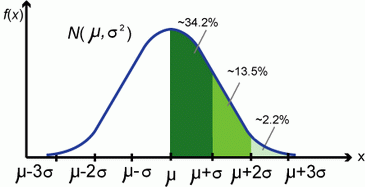
\includegraphics[keepaspectratio, scale=0.7]{no6.png}
  \caption{正太分布曲线\label{fig:no6}} 
\end{figure}
\par
符合正态分布概率计算的数学公式如下:
\begin{equation}\centering
  Pr=\frac{1}{\sqrt{2\pi}\sigma}e^{\frac{-(X-\mu)^{2}}{2\sigma^{2}}}
\end{equation}
\subsubsection{通过正太分布概率计算筛选移动设备定位范围}
当一个移动终端设备出现在该有限空间内时,这个设备所在的位置就是一个待定位点(LP)。该设备在LP上会收集到一组AP的信息,通过将这组AP信息和校准表上各CP中所有AP的离散值进行概率计算,便可以得到这个LP可能出现在每个CP上的概率值,而概率值最大的几个CP便可以确定该设备有可能出现在有限空间内的几个小区域。

\subsection{通过支持向量机计算待定位设备的准确位置}
\subsubsection{支持向量机(SVM)概念}
支持向量机(英语:Support Vector Machine,学术文献中常简称为SVM,中文简称则是“支持向量机”)是一种机器学习的方法,可广泛地应用于统计分类以及回归分析。
\par
支持向量机属于一般化线性分类器,也可以被认为是提克洛夫规范化(Tikhonov Regularization)方法的一个特例。这族分类器的特点是他们能够同时最小化经验误差与最大化几何边缘区,因此支持向量机也被称为最大边缘区分类器。
\par
支持向量机将向量映射到一个更高维的空间里,在这个空间里建立有一个最大间隔超平面。在分开数据的超平面的两边建有两个互相平行的超平面,分隔超平面使两个平行超平面的距离最大化。假定平行超平面间的距离或差距越大,分类器的总误差越小。
\subsubsection{支持向量机原理}
设样本属于两个类,用该样本训练svm得到的最大间隔超平面。在超平面上的样本点也称为支持向量。
\begin{enumerate}
\item 支持向量是相邻两类彼此最靠近的样本;
\item SVM即找出一个超平面,使两类相邻样本的间隔(margin)b最大,如图\ref{fig:no7}
  \begin{figure}[!ht]\centering
    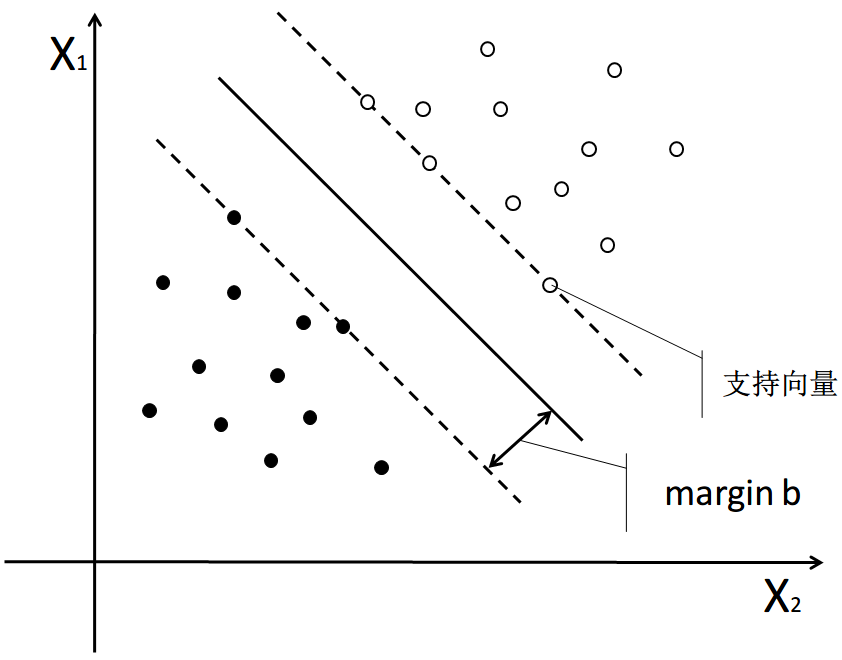
\includegraphics[keepaspectratio, scale=0.35]{no7.png}
    \caption{超平面分割样本空间\label{fig:no7}} 
  \end{figure}
\item 超平面的表达式:
  \begin{equation}
    g(x)=w^{t}x+w_{0}
  \end{equation}
  $w$为判决平面的权重向量,$w_{0}$为原点到平面的距离。
\item 假设系统线性可分,寻找一个分隔平面使得已经标记过的一组样本点$(x_{n},y_{n})$(其中$y_{n}$为标志位区分样本的类别),满足:
  \begin{equation}
    y_{k}g(x_{k})\geqslant b, \ \ \ b\geqslant0,k=1,...,n
  \end{equation}
\item 结构最小化风险函数就是在满足上式条件下最大化$b(margin)$。
\item 最终得到寻找最优超平面的方法如下:
  \begin{equation}
    min \ \ \ \frac{\|w\|^{2}}{2}
  \end{equation}
\item SVM就是利用训练样本找到满足上面约束的超平面,通过的数学手段就是拉格朗日求极值的二次最优化问题。公式如下
  \begin{equation}
    L(w,\alpha)=\frac{1}{2}\|w\|^{2}-\sum_{k=1}^{n}\alpha(y_{k}w^{t}x_{k}+w_{0}-1)
  \end{equation}
\item 由于$\|w\|^{2}$项的存在,这是一个二次优化计算,上面的函数为凸函数,故其存在唯一全局最优解。
\end{enumerate}

\subsubsection{RBF核函数}
当样本不是线性可分时,如图\ref{fig:no8}
\begin{figure}[!ht]\centering
  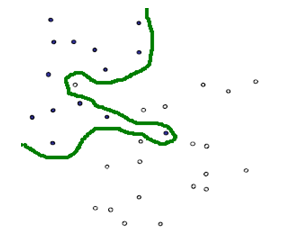
\includegraphics[keepaspectratio, scale=1]{no8.png}
  \caption{非线性样本空间\label{fig:no8}} 
\end{figure}
我们需要使用核函数,将非线性的样本映射到更高维的线性空间,之后才可以使用SVM方法进行超平面计算,从而分割样本类。
\par
RBF(径向基函数,也称高斯径向基函数)就是一个用来映射非线性样本的核函数,公式如下:
\begin{equation}
  K(x,z)=e^{\left(-\frac{\|x-z\|^{2}}{\sigma^{2}}\right)}
\end{equation}
通过使用核函数映射非线性样本,产生出了针对非线性样本的线性分类方法,得到如下公试:
\begin{equation}
  g(x)=\sum_{i=1}^{N_{s}}\alpha_{i}y_{i}K(x_{i},x)+w_{0}>(<)0
\end{equation}
$N_{s}$为支持向量的数量,$x_{i}$为输入的向量。

\subsubsection{不可分情形下的变形SVM}
当样本空间中不同类样本有重叠时,SVM必须引入松弛变量,将某些无法划分的样本也归入到支持向量中。因此使用一个叫惩罚因子的数学方法实现,原来的优化问题就变成了下面这样:
\begin{equation}
  min \ \ \ \frac{\|w\|^{2}}{2}+C\sum_{i=1}^{l}\zeta_{i}
\end{equation}
\begin{equation}
  subject\ to\ y_{i}[(wx_{i})+b]\geqslant1-\zeta_{i}\ \ \ (i=1,2,...,l)
\end{equation}
其中$l$是样本数。
\begin{enumerate}
\item 并非所有的样本点都有一个松弛变量与其对应。
\item 松弛变量的值实际上标示出了对应的点到底离群有多远,值越大,点就越远。
\item 惩罚因子是松弛变量的具体实现方式。
\item 惩罚因子C决定了你有多重视离群点带来的损失。
\item 惩罚因子C不是一个变量,整个优化问题在解的时候,C是一个你必须事先指定的值。
\end{enumerate}

\subsubsection{用支持向量机定位移动设备精确位置}
得到了LP的大致方位,就可以采用支持向量机的数学模型来对移动设备进行精确定位。将概率最大的两个CP上有效的AP信息和他们所标示的位置一一对应,再将待定位移动设备上收集到的AP信息与这两组向量做支持向量机计算,并得到一个确定的对应位置,该位置就是这个移动设备出现在该有限空间内的相对准确位置。

\subsection{原理总结}
用概率计算,得到移动设备进行精确定位时所需数据,再用支持向量机计算移动设备的精确位置,可以避免软件进行大量的无效计算,也可以避免无效数据进入支持向量机的计算过程。通过概率计算的筛选,提高了WIFI定位过程的效率,也实现了概率与支持向量机计算的有效结合提高了定位准确性。

%%%%%%%%%%%%%%%%%%%%%%%%%%%%%%%%%%%%%%%%%%%%%%%

\section{方法}
本文阐述的技术实现方法,涉及到网络通讯、科学计算、数据库相关技术。服务器负责地图、位置信息、校准数据和科学计算等功能。移动设备软件负责收集AP信息、向服务器发送信息和接收服务器返回的位置结果。
\par
总体过程如图\ref{fig:no1}
\begin{figure}[!ht]\centering
  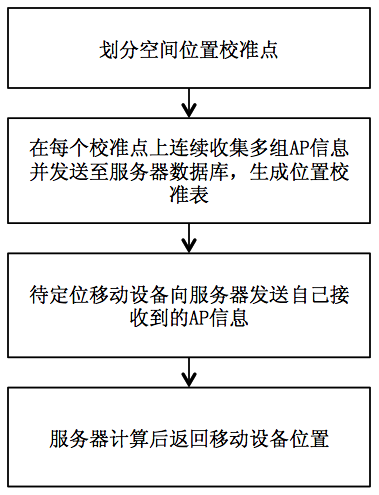
\includegraphics[keepaspectratio, scale=0.4]{no1.png}
  \caption{WIFI定位总体过程示意图\label{fig:no1}} 
\end{figure}

\subsection{有限空间的位置校准信息采样方法}
\begin{enumerate}
\item 确定一个有限空间的范围,将该空间内划分为多个小区域,每个小区域中确定一个WiFi定位校准点CP。
\item 用移动设备,在每个CP上采集AP信息,每次采集一组AP数据,同时发送到服务器端,保存至数据库。在同一个CP上,要连续多次采集AP数据,采集次数应该至少不低于5次。
\item 服务器端将所有CP上收集的AP信息,保存至数据库,将其中信号值为-100的AP信息去除,同时将AP出现次数少于2次的AP信息去除。
\item 生成WiFi定位原始数据采集表。
\end{enumerate}

\subsubsection{确定空间边界}
这个过程需要根据以下规则执行:
\begin{compactitem}
\item\textbf{确定有效的定位空间}
\item\textbf{确定无效的定位空间}
\item\textbf{有效定位空间域和无效定位空间的边界,就是最终定位空间的边界}
\item\textbf{将无效定位空间全部忽略,只记录所有有效定位空间的布局图}
\end{compactitem}
\par
如图\ref{fig:no2},图形区域之外的范围都是定位无效空间
\begin{figure}[!ht]\centering
  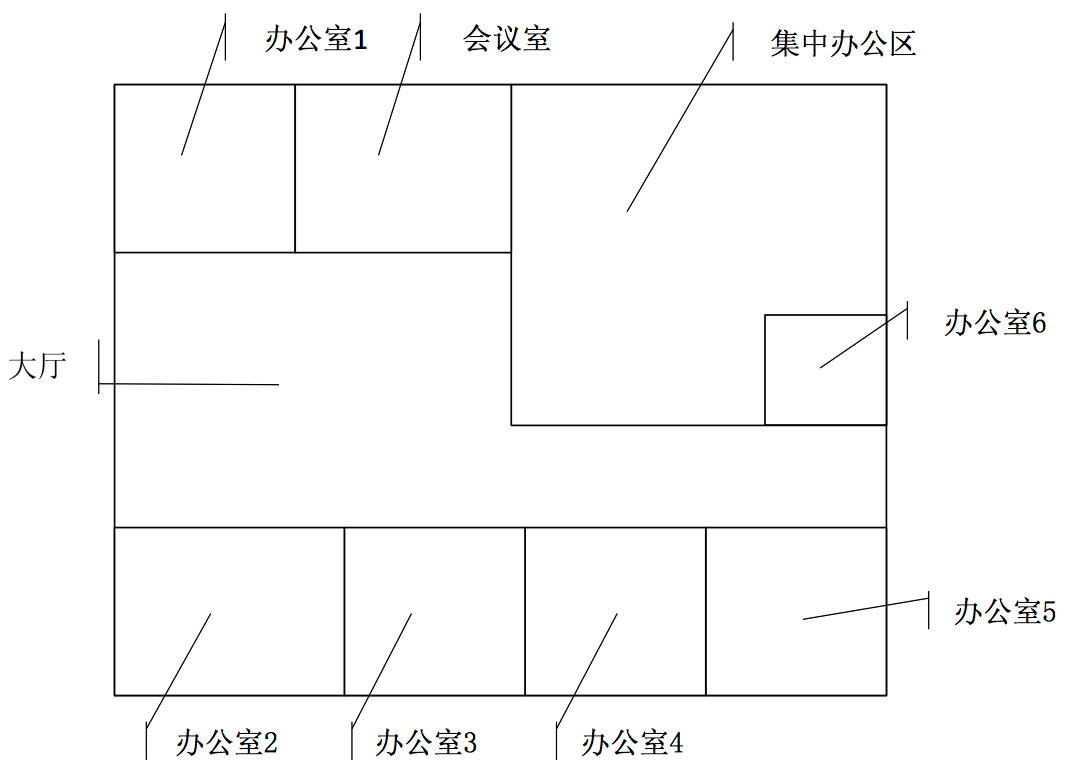
\includegraphics[keepaspectratio, scale=0.2]{no2.png}
  \caption{确定空间边界示意图\label{fig:no2}} 
\end{figure}

\subsubsection{划分位置区域}
在确定空间边界后,将这个空间根据实际定位需求,划分为多个小区域。实际定位需求,指的就是WiFi定位的目的,必须根据实际空间的状态来划分。通常做法是将空间内的有效使用空间划分为小区域,比如确定一层写字楼为一个需要定位的空间,那么根据实际应用需求,可以将每个办公室或大房间中的每个工作区,划分为小区域。示例如图\ref{fig:no3}
\begin{figure}[!ht]\centering
  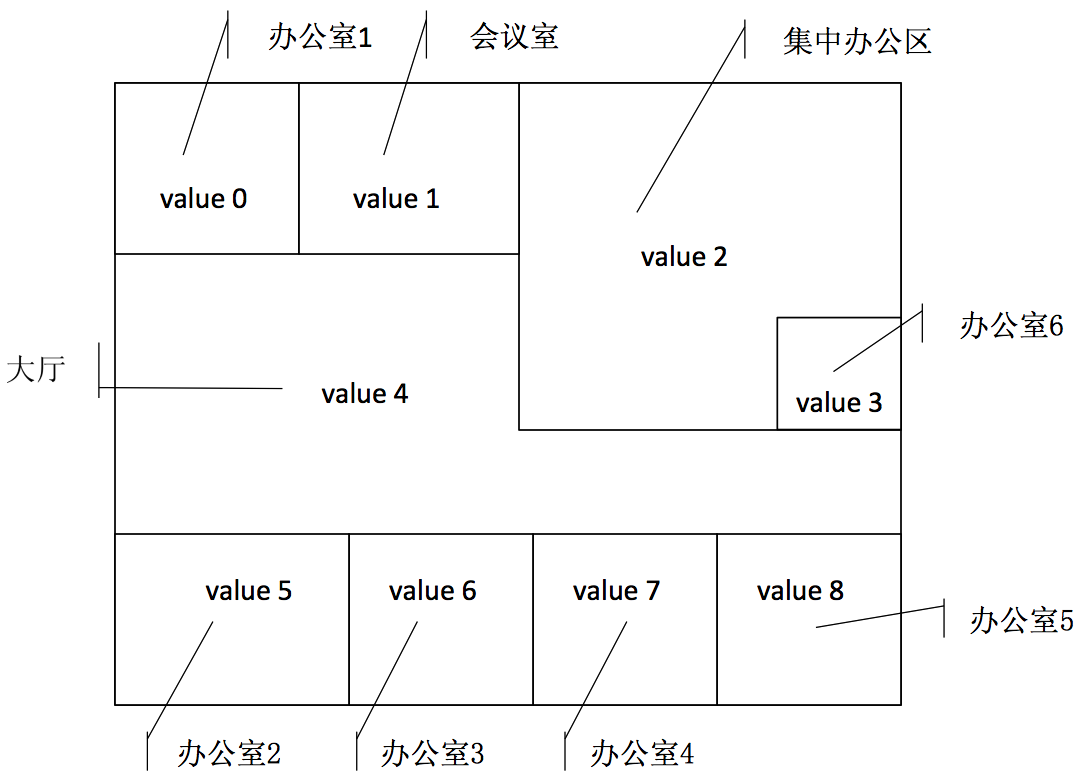
\includegraphics[keepaspectratio, scale=0.2]{no3.png}
  \caption{划分位置区域示意图\label{fig:no3}} 
\end{figure}

\subsubsection{确定每个区域中的位置校准点CP}
在划分好的小区域中,选择该区域的相对空间中心点,作为WiFi定位校准点CP。示例如图\ref{fig:no4}
\begin{figure}[!ht]\centering
  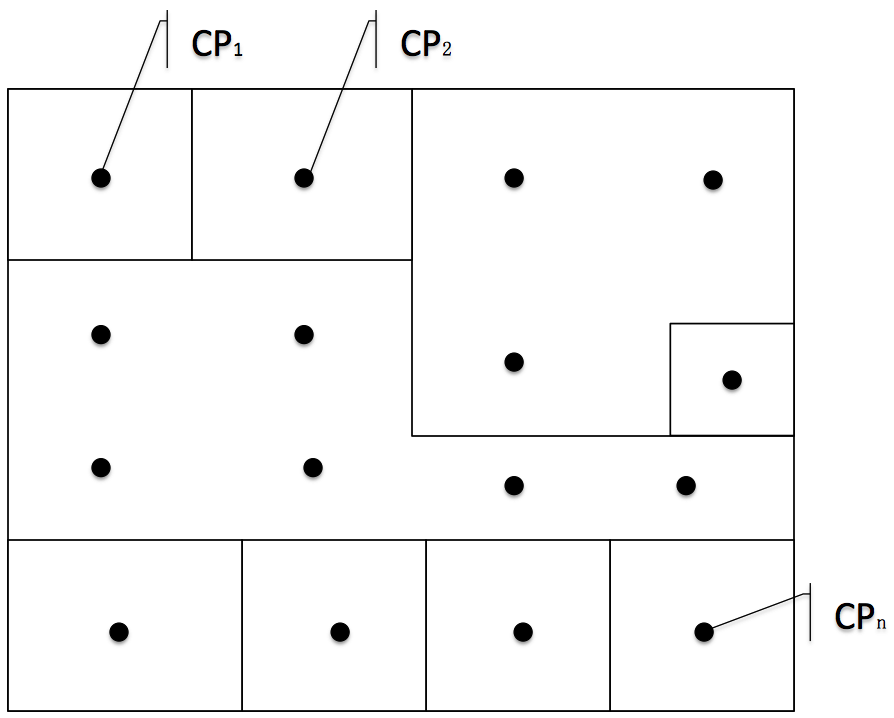
\includegraphics[keepaspectratio, scale=0.2]{no4.png}
  \caption{确定位置校准点示意图\label{fig:no4}} 
\end{figure}

\subsubsection{在每个CP上采集多组AP信息}
用一台移动终端设备,在每个CP上采集AP信息。每次采集会得到一组AP数据,其中有效数据,是每个AP的MAC地址和每个AP的信号值,为了之后处理数据,还必须同时保存采集数据的时间点,每次采集的一组AP,和采集时间点一一对应,发送至数据库保存。数据库中的最终数据如图\ref{fig:no5}:
\begin{figure}[!ht]\centering
  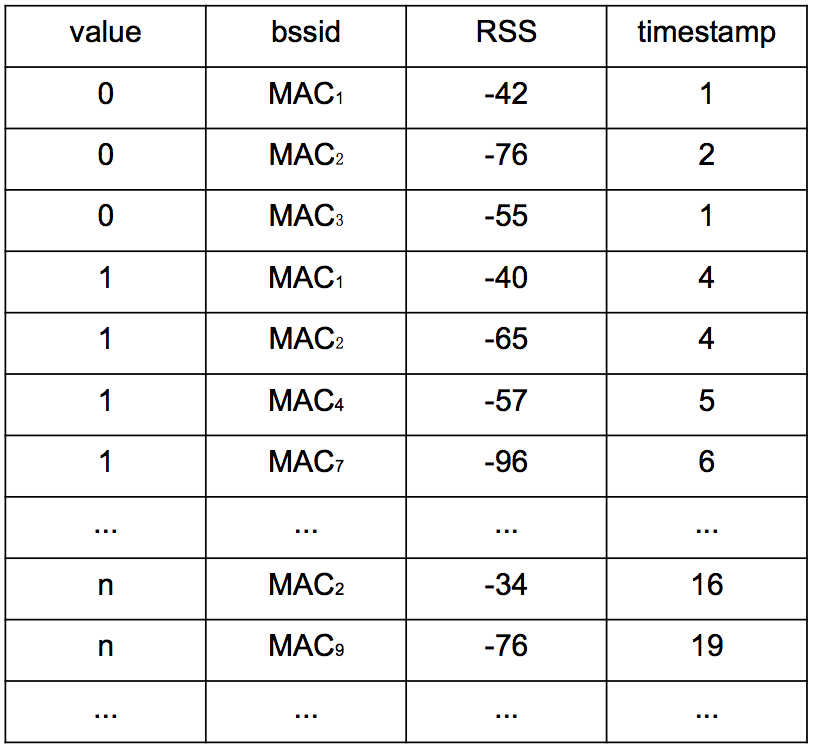
\includegraphics[keepaspectratio, scale=0.26]{no5.png}
  \caption{最终定位原始数据表示意图\label{fig:no5}} 
\end{figure}
\begin{compactitem}
\item\textbf{value}:定位区域ID
\item\textbf{bssid}:AP的MAC地址
\item\textbf{RSS}:AP的信号值
\item\textbf{timestamp}:采样时间点
\end{compactitem}

\subsection{建立位置校准表}
根据原始数据表,建立位置校准表。位置校准表,是WiFi定位功能的核心数据表,根据校准数据表的计算实现最终定位目的。
\par
位置校准表是对原始数据表中,每个区域每次采集到的AP,处理后得到,有效信息是区域ID(value)、AP的MAC地址(bssid)、AP的信号平均值(mRSS)、AP的信号离散度($\sigma$)。具体步骤如下:
\begin{compactitem}
\item\textbf{从原始数据表中,查出有效定位空间中所有的区域ID(CP value)。}
\item\textbf{根据CP value,查出每个区域中采样得到的所有AP信息}
\item\textbf{根据AP出现的次数和每次AP的信号值(RSS),计算得出每个AP在该CP中的信号平均值(mRSS)}
\item\textbf{根据单个AP信号的各个RSS,和该AP的信号mRSS,计算出该AP的信号方差($\sigma^{2}$)}
\item\textbf{将每个AP对应的CP value、AP的MAC地址(bssid)、mRSS、$\sigma^{2}$,存入数据库,形成定位校准表}
\end{compactitem}

\subsubsection{计算AP信号物理值}
计算AP信号的平均值,必须将原始数据中,AP信号指数值计算成物理值。移动设备接收到的AP信号值,都是物理值以10位底的对数,单位是dbm。dbm与物理信号值的换算公式如下:
\begin{equation}
  RSS=10\lg{P}
\end{equation}
P为WiFi发射功率,单位:瓦特(w)。由此公式可得物理信号的计算方法:
\begin{equation}
  P=10^{\frac{RSS}{10}}
\end{equation}

\subsubsection{计算CP中所有AP信号平均值和标准差}
计算AP的信号平均值,首先要将AP每次采集到的信号指数值换算成物理信号值,再将这些信号物理值相加,并除以该AP出现的次数。如果一个CP中采集到的一个AP共出现了N次,那么这个AP的限号平均值计算方法如下:
\begin{equation}
  mRSS=10\lg\left(\frac{1}{N}\sum^{N}_{i=1}10^{\frac{RSS_{i}}{10}}\right)
\end{equation}
得到AP的信号平均值后,就可以计算出该AP的信号离散度,也就是该AP信号的方差($\sigma^{2}$)和标准差($\sigma$),具体计算公式如下:
\begin{equation}
  \sigma^{2}=\frac{1}{N-1}\sum^{N}_{i=1}\left(mRSS-RSS_{i}\right)^{2}
\end{equation}
标准差是方差的算术平方根,两者都代表一组数据的相对离散程度,在具体的概率计算中各自的使用有细微差别。基于正态分布的概率计算中,方差和标准差都可以使用。

\subsubsection{生成校准表}
总结校准表的生成过程,以下图组可以表示:

\begin{enumerate}
\item 从原始数据表中查找出,在每个CP上收集到的AP信息。
  \begin{equation}
    \begin{array}{c|c}
      CP_{value} & AP_{i} \\ \hline
      CP_{0} & MAC_{1} \\
      CP_{0} & MAC_{2} \\
      CP_{0} & MAC_{3} \\
      CP_{0} & MAC_{4} \\
      CP_{0} & MAC_{5} \\
      ... & ...
    \end{array}
  \end{equation}
\item 根据CP和AP的MAC地址信息,查找出每个AP在一个CP上收集到的所有信号值。
  \begin{equation}
    \begin{array}{c|c|c}
      CP_{value} & AP_{i} & RSS_{(i,j)} \\ \hline
      CP_{0} & MAC_{1} & RSS_{(1,1)}...RSS_{(1,i)} \\
      CP_{0} & MAC_{2} & RSS_{(2,1)}...RSS_{(1,i)} \\
      CP_{0} & MAC_{3} & RSS_{(3,1)}...RSS_{(1,i)} \\
      CP_{0} & MAC_{4} & RSS_{(4,1)}...RSS_{(1,i)} \\
      CP_{0} & MAC_{5} & RSS_{(5,1)}...RSS_{(1,i)} \\
      ... & ... & ...
    \end{array}
  \end{equation}
\item 计算出每个AP在一个CP上的信号平均值。
  \begin{equation}
    \begin{array}{c|c|c}
      CP_{value} & AP_{i} & mRSS_{i} \\ \hline
      CP_{0} & MAC_{1} & mRSS_{1} \\
      CP_{0} & MAC_{2} & mRSS_{2} \\
      CP_{0} & MAC_{3} & mRSS_{3} \\
      CP_{0} & MAC_{4} & mRSS_{4} \\
      CP_{0} & MAC_{5} & mRSS_{5} \\
      ... & ... & ...
    \end{array}
  \end{equation}
\item 根据每个AP在一个CP上的信号平均值,和这个AP在该CP上的所有信号原值,计算出该AP在该CP上的信号值离散度方差。
  \begin{equation}
    \begin{array}{c|c|c|c}
      CP_{value} & AP_{i} & mRSS_{i} & \sigma^{2}_{i} \\ \hline
      CP_{0} & MAC_{1} & mRSS_{1} & \sigma^{2}_{1} \\
      CP_{0} & MAC_{2} & mRSS_{2} & \sigma^{2}_{2} \\
      CP_{0} & MAC_{3} & mRSS_{3} & \sigma^{2}_{3} \\
      CP_{0} & MAC_{4} & mRSS_{4} & \sigma^{2}_{4} \\
      CP_{0} & MAC_{5} & mRSS_{5} & \sigma^{2}_{5} \\
      ... & ... & ... & ...
    \end{array}
  \end{equation}
\item 将每个AP的MAC地址信息、该AP的信号平均值、该AP的信号离散度方差和该AP的校准点信息(CP),全部存入数据库中,建立一个新数据表——校准表。
  \begin{equation}
    \begin{array}{c|c|c|c}
      CP_{value} & AP_{i} & mRSS_{i} & \sigma^{2}_{i} \\ \hline
      CP_{0} & MAC_{1} & mRSS_{1} & \sigma^{2}_{1} \\
      CP_{0} & MAC_{2} & mRSS_{2} & \sigma^{2}_{2} \\
      CP_{0} & MAC_{3} & mRSS_{3} & \sigma^{2}_{3} \\
      ... & ... & ... & ... \\
      CP_{1} & MAC_{1} & mRSS_{1} & \sigma^{2}_{1} \\
      CP_{1} & MAC_{2} & mRSS_{2} & \sigma^{2}_{2} \\
      CP_{1} & MAC_{3} & mRSS_{3} & \sigma^{2}_{3} \\
      ... & ... & ... & ... \\
      CP_{2} & MAC_{1} & mRSS_{1} & \sigma^{2}_{1} \\
      CP_{2} & MAC_{2} & mRSS_{2} & \sigma^{2}_{2} \\
      CP_{2} & MAC_{3} & mRSS_{3} & \sigma^{2}_{3} \\
      ... & ... & ... & ...
    \end{array}
  \end{equation}
\end{enumerate}

\subsection{移动设备WiFi定位过程}
完成定位校准表之后,当一个待定位移动设备出现在有效定位空间内,该设备所处的位置,就是一个待定位点(LP),在该LP上会实时接收到一组AP信息,将这组AP信息发送到服务器端,服务器就根据校准表,对LP接收到的AP信息做正态概率计算,最后筛选出两个概率最大的CP信息。
\par
将筛选出的CP数据,和LP发送来的AP数据,做支持向量机计算,得到一个向量集对应的位置ID,该ID就是LP在有效定位空间内的具体位置。
\subsubsection{通过正态分布概率计算筛选有效CP}
\begin{enumerate}
\item 移动设备在LP上某一时刻接收到的AP信息如下:
  \begin{equation}
    \begin{array}{c|c}
      AP_{i} & RSS_{i} \\ \hline
      MAC_{1} & RSS_{1} \\
      MAC_{2} & RSS_{2} \\
      MAC_{3} & RSS_{3} \\
      MAC_{4} & RSS_{4} \\
      MAC_{5} & RSS_{5} \\
      MAC_{6} & RSS_{6}
    \end{array}
  \end{equation}
\item 从校准表中,CP值为查找条件,读取出一个CP对应的一组AP信息,如下:
  \begin{equation}
    \begin{array}{c|c|c|c}
      CP_{value} & AP_{i} & mRSS_{i} & \sigma^{2}_{i} \\ \hline
      CP_{0} & MAC_{1} & mRSS_{1} & \sigma^{2}_{1} \\
      CP_{0} & MAC_{2} & mRSS_{2} & \sigma^{2}_{2} \\
      CP_{0} & MAC_{3} & mRSS_{3} & \sigma^{2}_{3} \\
      CP_{0} & MAC_{4} & mRSS_{4} & \sigma^{2}_{4} \\
      CP_{0} & MAC_{5} & mRSS_{5} & \sigma^{2}_{5} \\
      ... & ... & ... & ...
    \end{array}
  \end{equation}
\item 查询移动设备提交的信息,和校准表中读取出的信息,找到MAC地址一致的AP和该AP的信号值,做正态分布概率计算,计算公式如下:
  \begin{equation}
    Pr_{i}=\frac{1}{\sqrt{2\pi}\sigma_{i}}e^{\frac{-(RSS_{i}-mRSS_{i})^{2}}{2\sigma_{i}^{2}}}
  \end{equation}
\item 将计算各个AP得到的概率值相加,最终得到该移动设备所在的LP,可能出现在该CP上的概率。
\item 重复第2、3、4步动作,将校准表中每个CP对应的AP信息,都按以上三个步骤做正态分布概率计算。最后得到该移动设备的LP,可能出现在所有CP上的概率。
\item 将得到的所有概率值排序,找到概率最大的两个CP,进入支持向量机的计算过程。
\end{enumerate}

\subsubsection{通过支持向量机计算LP在空间内的位置}
\begin{enumerate}
\item 根据之前通过正态分布概率计算,得到的两个概率最大的CP信息,从校准表中分别读取到这两个CP所对应的AP信息,按CP分为两组,如下图:
  \begin{equation}
    \begin{array}{c|c|c|c}
      CP_{value} & AP_{i} & mRSS_{i} & \sigma^{2}_{i} \\ \hline
      CP_{a} & MAC_{1} & mRSS_{1} & \sigma^{2}_{1} \\
      CP_{a} & MAC_{2} & mRSS_{2} & \sigma^{2}_{2} \\
      CP_{a} & MAC_{3} & mRSS_{3} & \sigma^{2}_{3} \\
      CP_{a} & MAC_{4} & mRSS_{4} & \sigma^{2}_{4} \\
      CP_{a} & MAC_{5} & mRSS_{5} & \sigma^{2}_{5} \\
      ... & ... & ... & ...
    \end{array}
  \end{equation}
  和
  \begin{equation}
    \begin{array}{c|c|c|c}
      CP_{value} & AP_{i} & mRSS_{i} & \sigma^{2}_{i} \\ \hline
      CP_{b} & MAC_{1} & mRSS_{1} & \sigma^{2}_{1} \\
      CP_{b} & MAC_{2} & mRSS_{2} & \sigma^{2}_{2} \\
      CP_{b} & MAC_{3} & mRSS_{3} & \sigma^{2}_{3} \\
      CP_{b} & MAC_{4} & mRSS_{4} & \sigma^{2}_{4} \\
      CP_{b} & MAC_{5} & mRSS_{5} & \sigma^{2}_{5} \\
      ... & ... & ... & ...
    \end{array}
  \end{equation}
\item 将移动设备在LP上采集到的AP信息,与以上两个CP中的AP信息,以相同MAC地址为条件做交集,得到一组AP的向量。
  \par
  $CP_{a}$的向量:
  \begin{equation}
    \begin{array}{c|c}
      AP_{i} & mRSS_{i} \\ \hline
      MAC_{1} & mRSS_{1} \\
      MAC_{3} & mRSS_{3} \\
      MAC_{5} & mRSS_{5} \\
      ... & ...
    \end{array}
  \end{equation}
  \par
  $CP_{b}$的向量:
  \begin{equation}
    \begin{array}{c|c}
      AP_{i} & mRSS_{i} \\ \hline
      MAC_{1} & mRSS_{1} \\
      MAC_{2} & mRSS_{2} \\
      MAC_{4} & mRSS_{4} \\
      ... & ...
    \end{array}
  \end{equation}
  \par
  移动设备在LP上采集到的AP向量:
  \begin{equation}
    \begin{array}{c|c}
      AP_{i} & mRSS_{i} \\ \hline
      MAC_{1} & mRSS_{1} \\
      MAC_{2} & mRSS_{2} \\
      MAC_{3} & mRSS_{3} \\
      ... & ...
    \end{array}
  \end{equation}
\item 分别将这两个CP的向量与该CP的value值对应:
  \begin{equation}
    \left(
    \begin{array}{c|c}
      AP_{i} & mRSS_{i} \\ \hline
      MAC_{1} & mRSS_{1} \\
      MAC_{3} & mRSS_{3} \\
      MAC_{5} & mRSS_{5} \\
      ... & ...
    \end{array}
    \right)CP_{a}
  \end{equation}
  \begin{equation}
    \left(
    \begin{array}{c|c}
      AP_{i} & mRSS_{i} \\ \hline
      MAC_{1} & mRSS_{1} \\
      MAC_{2} & mRSS_{2} \\
      MAC_{4} & mRSS_{4} \\
      ... & ...
    \end{array}
    \right)CP_{b}
  \end{equation}
\item 将3中整理得到的向量,输入SVM进行训练,如图\ref{fig:no9}所示:
  \begin{figure}[!ht]\centering
    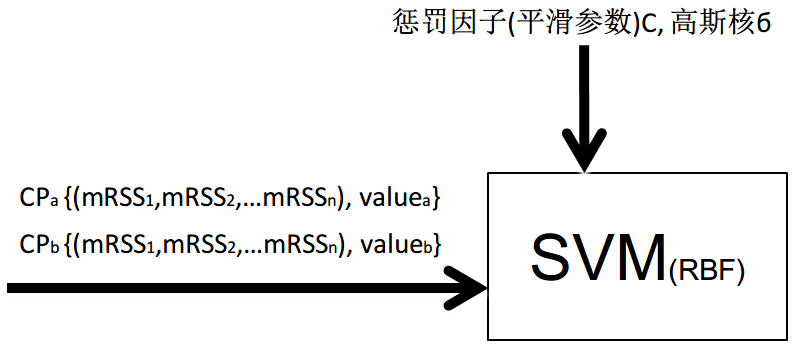
\includegraphics[keepaspectratio, scale=0.35]{no9.png}
    \caption{输入CP数据训练SVM\label{fig:no9}} 
  \end{figure}
\item 最后将移动设备在LP上采集到的AP向量,SVM(RBF)计算,最终得到其中一个CP的value值。如图\ref{fig:no10}所示:
  \begin{figure}[!ht]\centering
    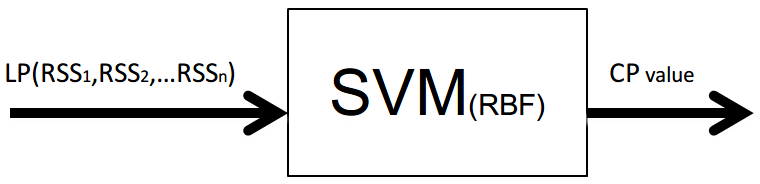
\includegraphics[keepaspectratio, scale=0.35]{no10.png}
    \caption{输入LP数据得到SVM的分类结果\label{fig:no10}} 
  \end{figure}
\end{enumerate}
\par
至此,移动设备定位过程结束。最终得到的这个CP的value值,所对应的有效定位空间位置(对应于图\ref{fig:no3}),就是该移动设备所在的空间位置。

%%%%%%%%%%%%%%%%%%%%%%%%%%%%%%%%%%%%%%%%%%%%%%

\section{结果}
采用正态分布概率计算,将移动设备的位置范围缩小至两个CP,再通过支持向量机在这两个CP中确定一个准确位置。
\par
完整的系统,要包括移动设备终端程序和服务器程序,这两个程序分别实现数据采集和数据处理的功能。
\subsection{移动设备终端程序}
负责收集空间内所采集到的AP信息。每次采集一组,向服务器提交数据,也按照一次采集的一组AP信息。采集AP信息的目的有两个:为了服务器生成校准数据;为了移动设备自身定位。
\subsubsection{为生成校准表所采集的数据}
此类数据按CP划分,每个CP上都要采集多组(一组为一次采集到的所有AP)。采集到的数据,必须标明CP value值后,才能提交给服务器端数据库,数据库按CP value的值作为查找条件建立数据表,存储数据。
\subsubsection{为自身定位所采集的数据}
此类数据都是实时的,某一时刻采集到的所有AP信息作为一次采集,定位也只需要一次采集的数据。此类数据不需要存储。
\subsection{系统训练}
训练过程是定位过程的前提条件,主要内容是校准表的建立,和SVM特征向量训练。
\subsubsection{建立校准表}
收集完成所有CP的原始采样信息后,就可以建立校准表,校准表是进行概率计算的前提,需要在所有定位操作之前完成。校准表的建立,也是要将CP value值作为查找条件,未来的概率计算依靠的就是CP value值作为数据单元的读取条件。
\subsubsection{SVM特征向量训练}
在移动设备定位过程中,当概率计算完成后,缩小定位区域在两个CP中。当要使用SVM在这两个CP中实现精确定位,首先需要将这两个CP的特征向量(CP在校准表中的信息)进行训练。

\subsection{移动设备定位}
完成校准表后,系统就可以开始进行移动设备的定位服务。当一个设备将一次收集到的AP信息提交给服务器后,服务器从校准表中按CP值为查找条件,依次读取每个CP所包含的AP校准数据。将这些读出的数据分别和移动设备提交的AP数据做概率计算,以CP值为区分条件,将一个CP中计算出的所有概率相加,最后找到两个概率和最大的CP。
\par
将概率计算得出的这两个CP的value,作为查找条件,从校准表中读出CP所对应的内容。将这些内容与CP的value值一一对应,制作成向量集,输入SVM进行机器学习训练。完成训练后,再将移动设备提交的这组AP信息输入SVM,从而得到一个CP value,这个值就表示移动设备经过系统定位计算后,最终的精确位置。

%%%%%%%%%%%%%%%%%%%%%%%%%%%%%%%%%%%%%%%%%%%%%%

\section{技术创新(权利保护)}
\subsection{用边界入口点校准的方法解决WiFi定位功能开关和不同类型设备识别的问题}
本文所阐述的WiFi定位技术,在实际使用的过程中,首先会出现两个必须解决的问题:
\begin{enumerate}
\item 移动终端设备如何判断自身是否进入了一个可定位的空间,并开启定位服务?
\item 移动终端设备如何才能让定位系统知道自身的设备类型?
\end{enumerate}
\par
为了解决以上问题,我们采用边界入口点校准的方法实现。在定位空间的边界上,设置一个或多个入口校准点,所有需要WiFi定位服务的移动终端设备,都必须先到这些入口点进行校准。校准方式有很多种,如手动开启WiFi定位应用,二维码扫描开启WiFi定位应用等。
\par
在开启移动终端设备WiFi定位应用的同时,由于入口校准点是事先约定好的,因此该校准点的定位区域数据也是相对固定的。根据移动终端设备在该点接收到的区域定位数据,就可以判断出这个移动终端设备的WiFi信号识别能力。不同类型的移动终端设备,对于同样的AP,信号强度识别结果是不同的,根据这个特点,便可以基本判断出与这个移动终端设备的最接近的设备类型。

\subsection{用分级校准数据解决不同种类型WiFi设备识别AP信号差异问题}
由于不同类型的移动终端设备,对于同样的AP,信号强度识别结果不同,而一组完整的校准数据是用一台移动终端设备采集的。因此使用一组校准数据,无法实现多种不同类型的移动终端设备,进行准确的WiFi定位。
\par
为了解决这个问题,必须准备多组校准数据,这些数据使用不同类型的移动终端设备进行采集,根据移动终端设备类型分组保存。
\par
当移动终端设备在边界入口点开启WiFi定位应用的同时,根据设备所采集到的入口点的定位区域数据,可以判断出移动终端设备的类型,再根据该移动终端设备类型选择相应的校准数据,最终实现准确的WiFi定位。

\subsection{用共有AP的方法解决SVM训练时AP在识别过程中缺失的问题}
所有移动终端设备,在每次识别AP时都不可能做到绝对准确,因此一台移动终端设备不同时刻识别到的定位区域数据可能会存在不一致的情况。
\par
为了解决以上问题,必须在每次定位时,采用带定位数据与校准数据交集的结果,动态的进行SVM训练,使每次SVM训练用的特征向量中的AP,和LP的特征数据中的AP保证一致。
\par
而每次定位都做SVM训练,计算量非常大,并且已知其中绝大部分计算都是无用的。因此在做SVM计算之前,我们采用概率的方式筛选出LP出现可能最大的两个定位区域。之后之针对这两个定位区域的校准数据做SVM计算,这样大大提高了计算效率,同时保证了定位结果的准确。


%%%%%%%%%%%%%%%%%%%%%%%%%%%%%%%%%%%%%%%%%%%%%%

\section{应用前景}
WiFi定位技术可以应用在多种领域,主要为行业提供室内定位基础服务。本文阐述的WiFi定位技术,不依赖特定硬件和特殊环境要求,部署应用方便灵活,成本低,可以结合多种具体的业务实现垂直服务。
\subsection{室内定位和导航}
室内定位和导航,是WiFi最主要的应用方式,也是最直接的服务提供模式。
\begin{enumerate}
\item 公共室内空间的位置服务,如商场、超市和大规模的综合购物中心。为了方便顾客找到所需商品位置,或快速找到某个区域(例如卫生间、出口、餐饮区,等等),结合WiFi定位和电子地图技术,实现顾客自身位置确定和导航服务功能。
\item 室内区域流量统计服务,如在商场、超市和大规模的综合购物中心,有时业主需要统计一段时间内,某个区域或所有区域的客流信息,或者某个客流最大的热点区域。结合WiFi定位和电子地图以及大数据技术,可以实现室内区域的流量统计,顾客使用移动设备上的WiFi定位客户端软件,经过的路径会推送至服务器,服务器端根据统计整理,最后分析出某个或所有区域的客流数据。
\end{enumerate}
\subsection{地理围栏}
地理围栏是一个新兴的移动互联网服务概念,其主要目的是实现互联网应用和移动设备位置信息的结合。
\begin{enumerate}
\item 设备位置开启移动应用。当移动设备进入某个特定区域后,便自动开启一些应用软件。这种服务适合应用在商场导购,医院就医指导,机场火车站等公共服务场所。
\item 特定移动应用的使用范围。移动设备上的某些软件,只能在某些特定的环境中才可以使用。这种服务适合公司企业,用来实现现代移动化的企业管理和自动化办公。当员工进入企业办公区域后,相关工作的信息服务和业务软件才可以工作,保证了企业数据的安全,也将企业管理简单有效的实现。
\end{enumerate}
\subsubsection{移动设备防盗}
某些非个人使用的移动设备,如餐厅的点餐设备,高级场馆的自助服务设备,都是为了本地服务存在的。为了防止个别人将其私自带出,又要实现该设备的自由使用,就必须采用一种防盗的技术做应用保证。本文阐述的WiFi定位技术,可以划出移动设备的安全范围,当设备离开这个安全区域后,便可以通过报警、监控和追踪等方式及时发现并处理。
\subsubsection{区域信息安全}
信息隔离,是信息安全中的一项重要内容,指信息内容与信息的有效区域之间的对应关系。采用本文阐述的WiFi定位技术,可以通过软件安全策略,规定信息的安全范围,当移动设备需要读取某些带有安全级别的数据时,会根据移动设备所处的位置进行操作合法性判断,当发现移动设备所处的位置不合法时,便会组织数据的读取。对于已经读取到的数据,当设备离开该数据的安全区域后,通过软件安全策略谁自动删除该数据,保证数据存在的有效范围与数据的安全范围一致。
\subsubsection{地理信息隔离}
移动设备的最大特点是可以随身携带,可以随时随地的产生数据,如照相、笔记、下载或应用软件生成数据。利用本文所阐述的WiFi定位技术,可以在产生数据的同时,将数据与其产生时的位置做关联。无论在以后的搜索查找,或是统计,位置信息会提供跟多的有效途径,版主使用者对数据的管理。也可以将数据的存储或显示方式,与位置信息关联,是某些数据只在特定位置区域是才可以被操作。
\subsection{游戏}
电子游戏的场景通常是虚拟的空间,但是随着技术的发展,电子游戏的实现也可以利用现实空间。本文阐述的WiFi定位技术,可以实现真实空间在设备上的体现,电子游戏的方式也就从单一的虚拟空间扩展到了真实空间,游戏玩家除了操作设备,还需要亲身行动来完成游戏。这样的组合不仅扩展了电子游戏的功能,甚至可以改变电子游戏的传统运行模式。
%%%%%%%%%%%%%%%%%%%%%%%%%%%%%%%%%%%%%%%%%%%%%%

\end{document}
